% !TeX program = xelatex
\documentclass[10pt]{article}
\usepackage[a4paper,landscape,margin=8mm]{geometry}
\usepackage{amsmath,amssymb,bm,graphicx,booktabs,array,xcolor}
\usepackage{newtxtext,newtxmath}
\usepackage{microtype}
\usepackage{fix-cm}
\usepackage[colorlinks=true,urlcolor=teal]{hyperref}
\definecolor{navy}{HTML}{152C46}
\definecolor{teal}{HTML}{007C83}
\definecolor{muted}{HTML}{526171}
\definecolor{pale}{HTML}{EAF4F3}
\definecolor{line}{HTML}{CFD8E0}
\pagestyle{empty}
\linespread{1.0}
\setlength{\parindent}{0pt}
\setlength{\parskip}{2pt}
\setlength{\abovedisplayskip}{2pt}
\setlength{\belowdisplayskip}{2pt}
\setlength{\abovedisplayshortskip}{2pt}
\setlength{\belowdisplayshortskip}{2pt}
\newcommand{\sect}[2]{\par\vspace{2pt}{\color{teal}\bfseries\fontsize{11}{13}\selectfont #1\quad #2}\par\vspace{1pt}{\color{line}\hrule}\vspace{2pt}}
\newcommand{\subhead}[1]{\par\vspace{2pt}{\bfseries\color{navy}#1}\par}
\newcommand{\smallnote}[1]{{\fontsize{7.1}{8.3}\selectfont\color{muted}#1\par}}
\newcommand{\takeaway}[1]{\par\vspace{3pt}\colorbox{pale}{\parbox{\dimexpr\linewidth-2\fboxsep}{\bfseries\color{teal}#1}}\par}
\newcommand{\posterheader}[3]{\colorbox{navy}{\parbox{\dimexpr\textwidth-2\fboxsep}{\vspace{3mm}\hspace{3mm}\begin{minipage}{\dimexpr\linewidth-6mm}\color{white}{\bfseries\fontsize{20}{22}\selectfont #1\par}\vspace{2mm}{\fontsize{10}{12}\selectfont #2\hfill #3}\end{minipage}\vspace{3mm}}}\par\vspace{4mm}}
\newcommand{\columnstart}{\begin{minipage}[t]{0.318\textwidth}\vspace{0pt}}
\newcommand{\columnend}{\end{minipage}}
\newcommand{\colsep}{\hfill}
\newcommand{\posterfooter}[1]{\par\vspace{3mm}{\color{line}\hrule}\vspace{1.5mm}{\fontsize{6.7}{8}\selectfont\color{muted}#1\par}}

\begin{document}
\fontsize{8.7}{10.3}\selectfont
\posterheader{Variable-Thrust, Variable-Mass Rockets}{From orbital trajectory planning to predictive control}{Applied Mathematical Methods | 2026}
\columnstart
\sect{01}{Problem \& physical model}
\textbf{Orbit insertion requires both altitude and velocity.} Near-Earth orbits enable observation, space experiments and subsequent missions. Reaching altitude without sufficient transverse speed yields a suborbital return.
\subhead{Vertical ascent and ideal propulsion}
For expelled mass $-\mathrm dm>0$ and constant effective exhaust speed $c$, momentum balance gives
\[
 m\,\mathrm dv=-c\,\mathrm dm+F_{\rm ext}\,\mathrm dt.
\]
Neglecting external forces and integrating yields the Tsiolkovsky equation:
\[
 \boxed{\Delta v_{\rm ideal}=c\ln(m_0/m_f)}.
\]
Impulse is $I_T=\int T\,\mathrm dt=c(m_0-m_f)$; velocity gain integrates $T/m$. Starting from rest with $r\ge r_0$, no random forcing and dissipative drag, ideal propulsion and orbital energy imply
\[
 \frac{m_0}{m_f}\ge\exp\!\left[\frac{\sqrt{2\mu/r_0-\mu/r_*}}{c}\right].
\]
The necessary mass ratio is at least \textbf{6.245} in the 600 km case; this bound is not sufficient for insertion.
\subhead{Earth-centered planar polar dynamics}
Define $u=\dot r$, $w=r\dot\theta$, $V=\sqrt{u^2+w^2}$, propellant flow $q=-\dot m\ge0$ and thrust $T=cq$.
\[
\begin{aligned}
 \dot r&=u,\qquad \dot\theta=w/r,\qquad \dot m=-q,\\
 \dot u&=\frac{w^2}{r}+\frac{cq\cos\alpha}{m}-\frac{\mu}{r^2}
 -\frac{kVu}{m}+a_{\varepsilon,r},\\
 \dot w&=-\frac{uw}{r}+\frac{cq\sin\alpha}{m}
 -\frac{kVw}{m}+a_{\varepsilon,\theta}.
\end{aligned}
\]
Here $k=\rho C_DA/2$ and $\rho=\rho_0e^{-(r-R_E)/H}$. Thrust follows $\alpha=\operatorname{atan2}(w,u)+\delta$ after a short initial vertical hold.
\[
 a_{\varepsilon,j}=\sigma_{0,j}(\rho/\rho_{\rm ref})\eta_j(t).
\]
\smallnote{Gaussian forcing is continuously interpolated with finite temporal correlation, not ideal white noise. The planar point-mass model omits Earth rotation, lift and attitude actuator dynamics.}
\columnend\colsep
\columnstart
\sect{02}{Planning \& feedback control}
\subhead{Two burns: PSO search + SQP refinement}
A suborbital burn, coast and circularization burn structure the search over thrust-angle nodes, flow rates and phase durations. PSO combines personal and neighborhood experience; SQP then refines terminal feasibility.
\[
 r_*=R_E+600\,\mathrm{km},\qquad v_c=\sqrt{\mu/r_*},
\]
\[
 J=\left(\frac{r_f-r_*}{s_h}\right)^2+
 \left(\frac{u_f}{s_u}\right)^2+
 \left(\frac{w_f-v_c}{s_w}\right)^2.
\]
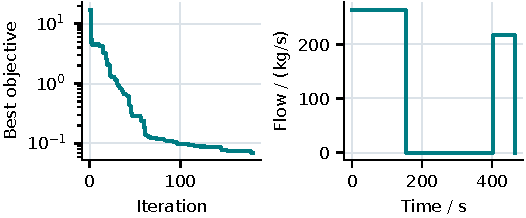
\includegraphics[width=\linewidth,height=31mm]{images/planning_en.pdf}
\smallnote{Left: PSO objective history. Right: final reference flow. Burn/coast/burn durations are approximately 153.3 / 250.0 / 62.0 s. Final accuracy reflects both PSO and local refinement.}
\subhead{Forward integration}
Runge--Kutta integration maps controls to trajectories. Batched GPU RK4 accelerates search; adaptive Dormand--Prince integration checks candidates with fuel-depletion and ground-impact events.
\subhead{MPC: measure, predict, solve, apply}
Track $x^{\rm ref}=(r,\theta,u,w,m)^\mathsf T$ using thrust-angle and flow corrections. Linearizing the discrete dynamics along the reference gives
\[
 e_{k+1}=A_ke_k+B_kv_k+d_k.
\]
Quadratic penalties on predicted tracking errors, control effort, control changes and slack variables are condensed into a convex quadratic program:
\[
 \min_\zeta\ \tfrac12\zeta^\mathsf TH\zeta+f^\mathsf T\zeta,
 \qquad G\zeta\le b.
\]
A \textbf{convex interior-point algorithm} solves the QP with angle, flow, dry-mass and ground constraints. Apply only the first correction, then repeat with fresh state feedback; retain the two-burn schedule.
\takeaway{Offline planning supplies a feasible reference; online MPC corrects disturbances in flight.}
\columnend\colsep
\columnstart
\sect{03}{600 km case \& findings}
\smallnote{$m_0=60\,000$ kg, $m_{\rm dry}=1\,200$ kg, $c=4\,500$ m/s. Open and closed loops share the same plant disturbance, distinct from the planning realization.}
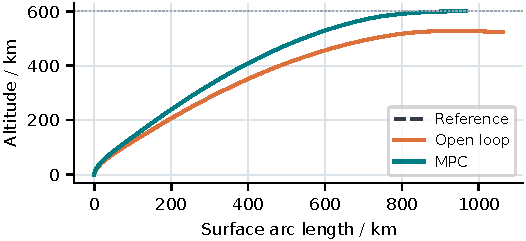
\includegraphics[width=\linewidth,height=36mm]{images/trajectory_en.pdf}
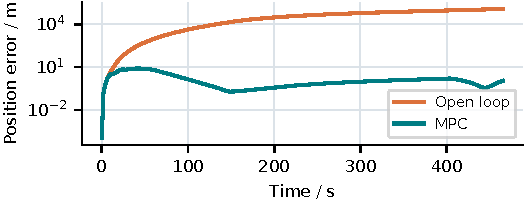
\includegraphics[width=\linewidth,height=30mm]{images/error_en.pdf}
\smallnote{MPC nearly overlaps the reference trajectory. Position error combines radial and surface-arc errors; zero values are floored only for logarithmic plotting.}
\vspace{2pt}
{\fontsize{8.1}{10.3}\selectfont
\setlength{\tabcolsep}{2pt}
\begin{tabular*}{\linewidth}{@{\extracolsep{\fill}}lrr@{}}
\toprule
Metric & Open loop & MPC\\\midrule
Position RMS / m & $5.98\times10^4$ & $2.606$\\
Velocity RMS / (m/s) & $298.084$ & $0.0992$\\
Cutoff altitude error / m & $-77\,611.6$ & $1.191$\\
Cutoff radial speed / (m/s) & $-557.983$ & $0.0231$\\
Tangential speed error / (m/s) & $233.256$ & $0.0559$\\\bottomrule
\end{tabular*}}
\smallnote{RMS is relative to the reference; cutoff errors are relative to the target circular orbit.}
\takeaway{Feedback suppresses error accumulation and brings cutoff close to circular-orbit conditions.}
\smallnote{Scope: one disturbance realization, ideal state feedback and a simplified atmosphere. No claim of global optimality, statistical robustness or proven closed-loop stability is made.}
\columnend
\posterfooter{References: NASA Glenn, Ideal Rocket Equation; Kennedy \& Eberhart, Particle Swarm Optimization, 1995; Dormand \& Prince, JCAM, 1980; Mayne et al., Automatica, 2000; Nocedal \& Wright, Numerical Optimization, 2006.\quad Data: project experiment snapshot, 20 Oct 2026.}
\end{document}
